\section{Final Tables for Tri-lepton Analyses}
A graphical comparison of the background estimations to be averaged is shown in detail in appendix~\ref{app:graphical}. 
Here, the summarized results are presented in five tables: 
\begin{itemize}
\item Table~\ref{tab:OSSF1tau0} contains observed yields  and background prediction 
for each search region in a tri-lepton channel with an opposite sign same flavor lepton pair present (3$\ell$).
\item Table~\ref{tab:OSSF0tau0}  - for a channel without  an opposite sign same flavor lepton pair (no OSSF).
\item Table~\ref{tab:SStau1} - for a channel with a same sign di-lepton and a hadronically decaying tau (SS$\tau$). 
This result is fully based on Ref.~\cite{AN2012:248}.
\item Table~\ref{tab:OSOFtau1} - for a channel with an opposite sign opposite flavor di-lepton and 
a hadronically decaying tau ($e^\pm\mu^\mp\tau$). This result is provided only in Ref.~\cite{AN2012:255}.
\item Table~\ref{tab:OSSF1tau1} - for a channel with an opposite sign same flavor di-lepton and 
a hadronically decaying tau (OSSF$\tau$). This result is based on Refs.~\cite{AN2012:255}~and~\cite{AN2012:256}.
\end{itemize}

The graphical representation of the combined results is shown in Figures~\ref{fig:OSSF1tau0},~\ref{fig:OSSF0tau0},
\ref{fig:SStau1},~\ref{fig:OSOFtau1},~\ref{fig:OSSF1tau1}.

%==========================================================================================
\begin{figure}[htp]
\begin{center}
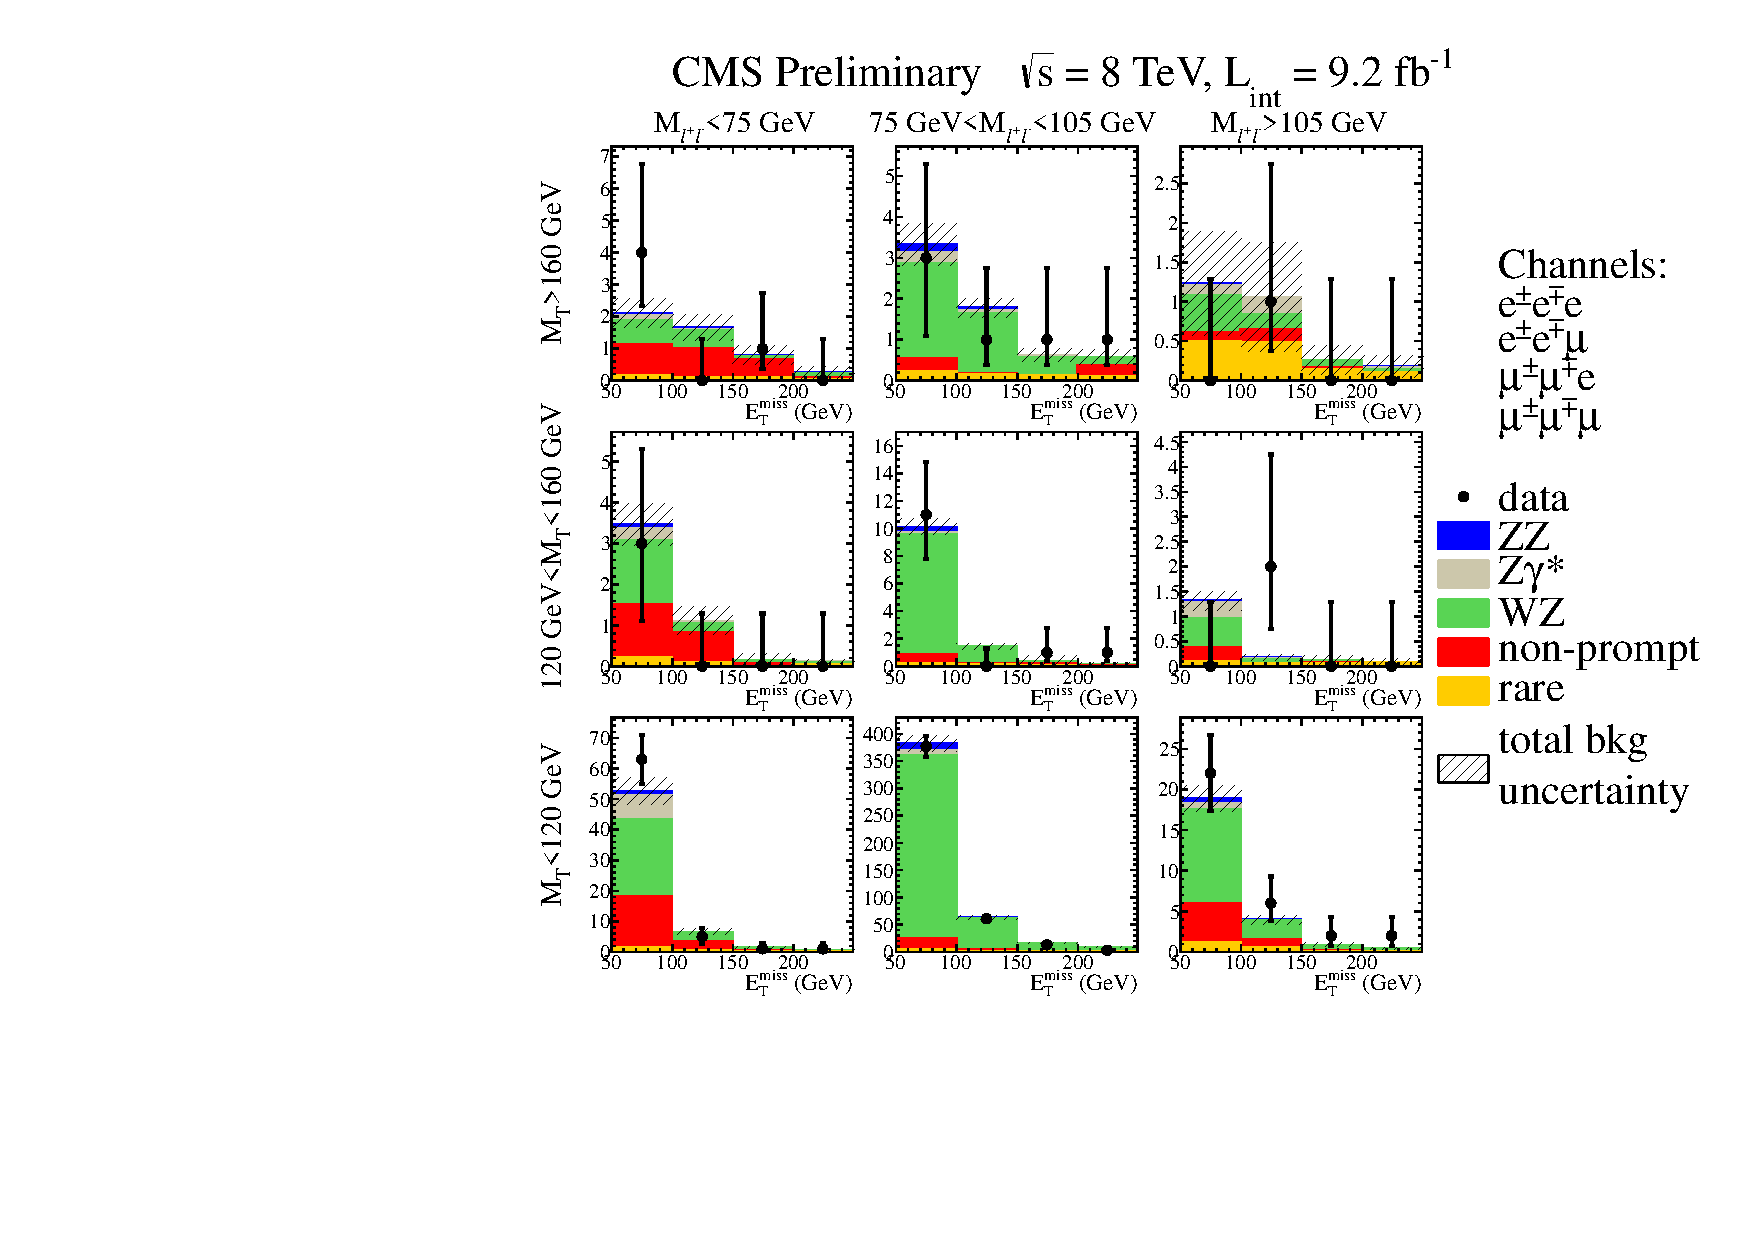
\includegraphics[width=1.0\textwidth]{plots/3lfinal/ossf1tau0.pdf}
\caption{Observed yields and predicted backgrounds for a tri-lepton with an opposite sign same flavor 
lepton pair present in all defined search regions.}
\label{fig:OSSF1tau0}
\end{center}
\end{figure}
%==========================================================================================
%==========================================================================================
\begin{figure}[htp]
\begin{center}
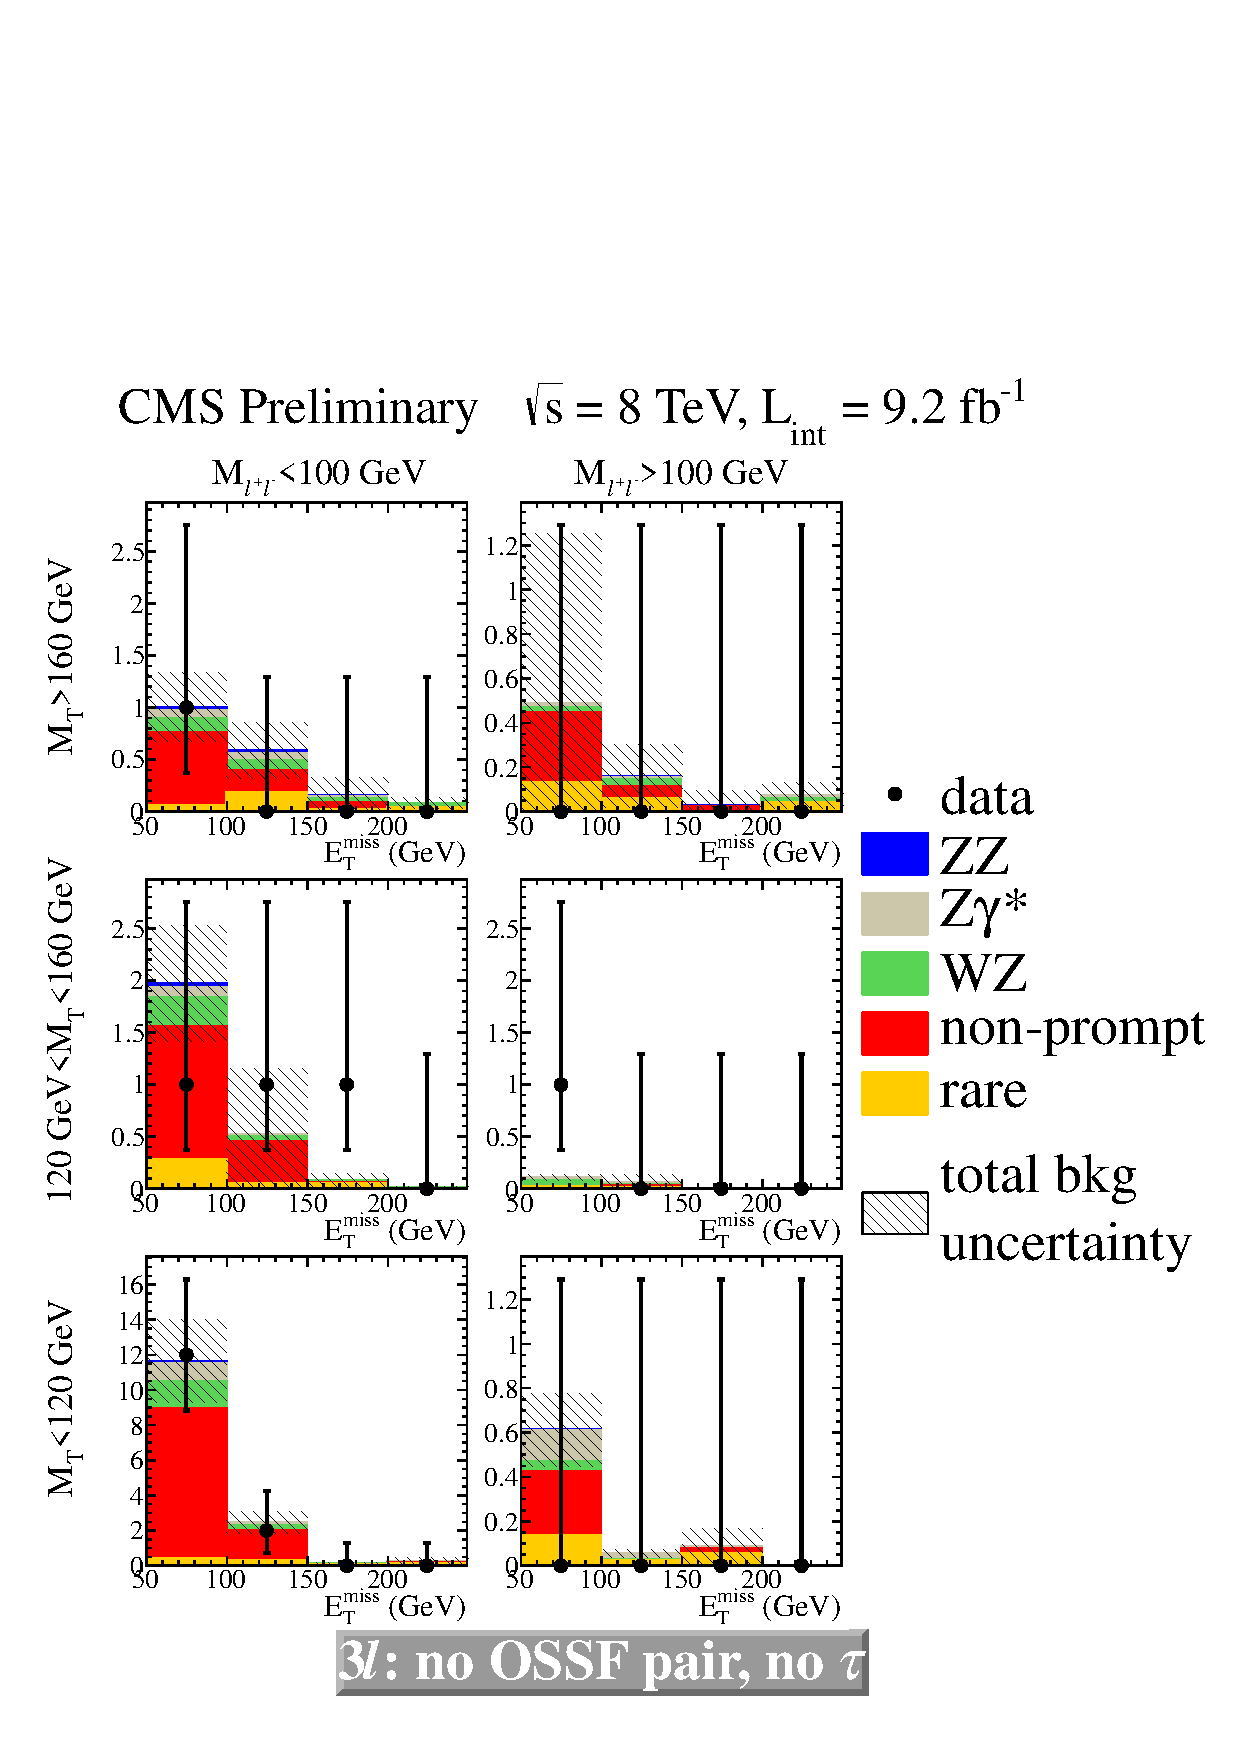
\includegraphics[width=1.0\textwidth]{plots/3lfinal/ossf0tau0.pdf}
\caption{Observed yields and predicted backgrounds for a tri-lepton without an opposite sign same flavor 
lepton pair present in all defined search regions.}
\label{fig:OSSF0tau0}
\end{center}
\end{figure}
%==========================================================================================
%==========================================================================================
\begin{figure}[htp]
\begin{center}
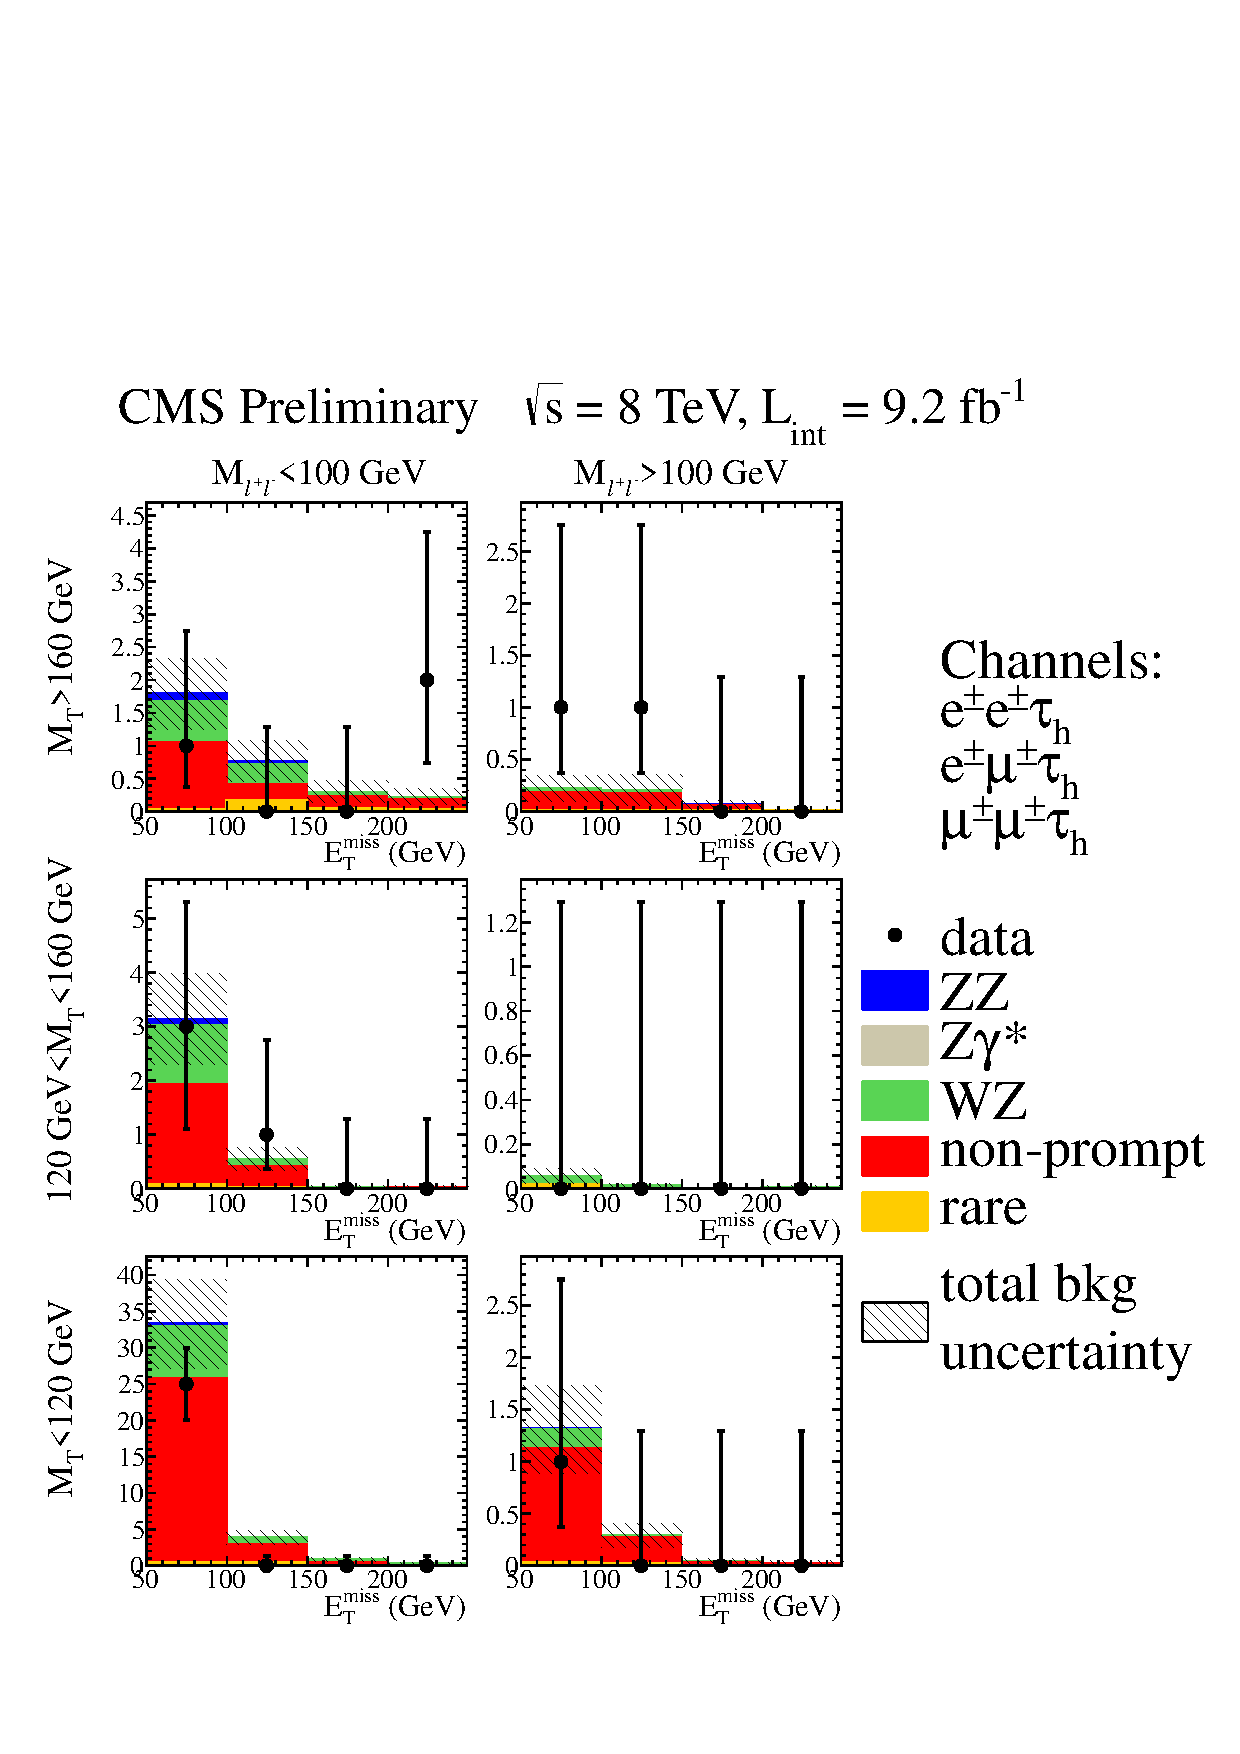
\includegraphics[width=1.0\textwidth]{plots/3lfinal/ossf0tau1.pdf}
\caption{Observed yields and predicted backgrounds for a tri-lepton with a same sign di-lepton 
and a hadronically decaying tau in all defined search regions.}
\label{fig:SStau1}
\end{center}
\end{figure}
%==========================================================================================
%==========================================================================================
\begin{figure}[htp]
\begin{center}
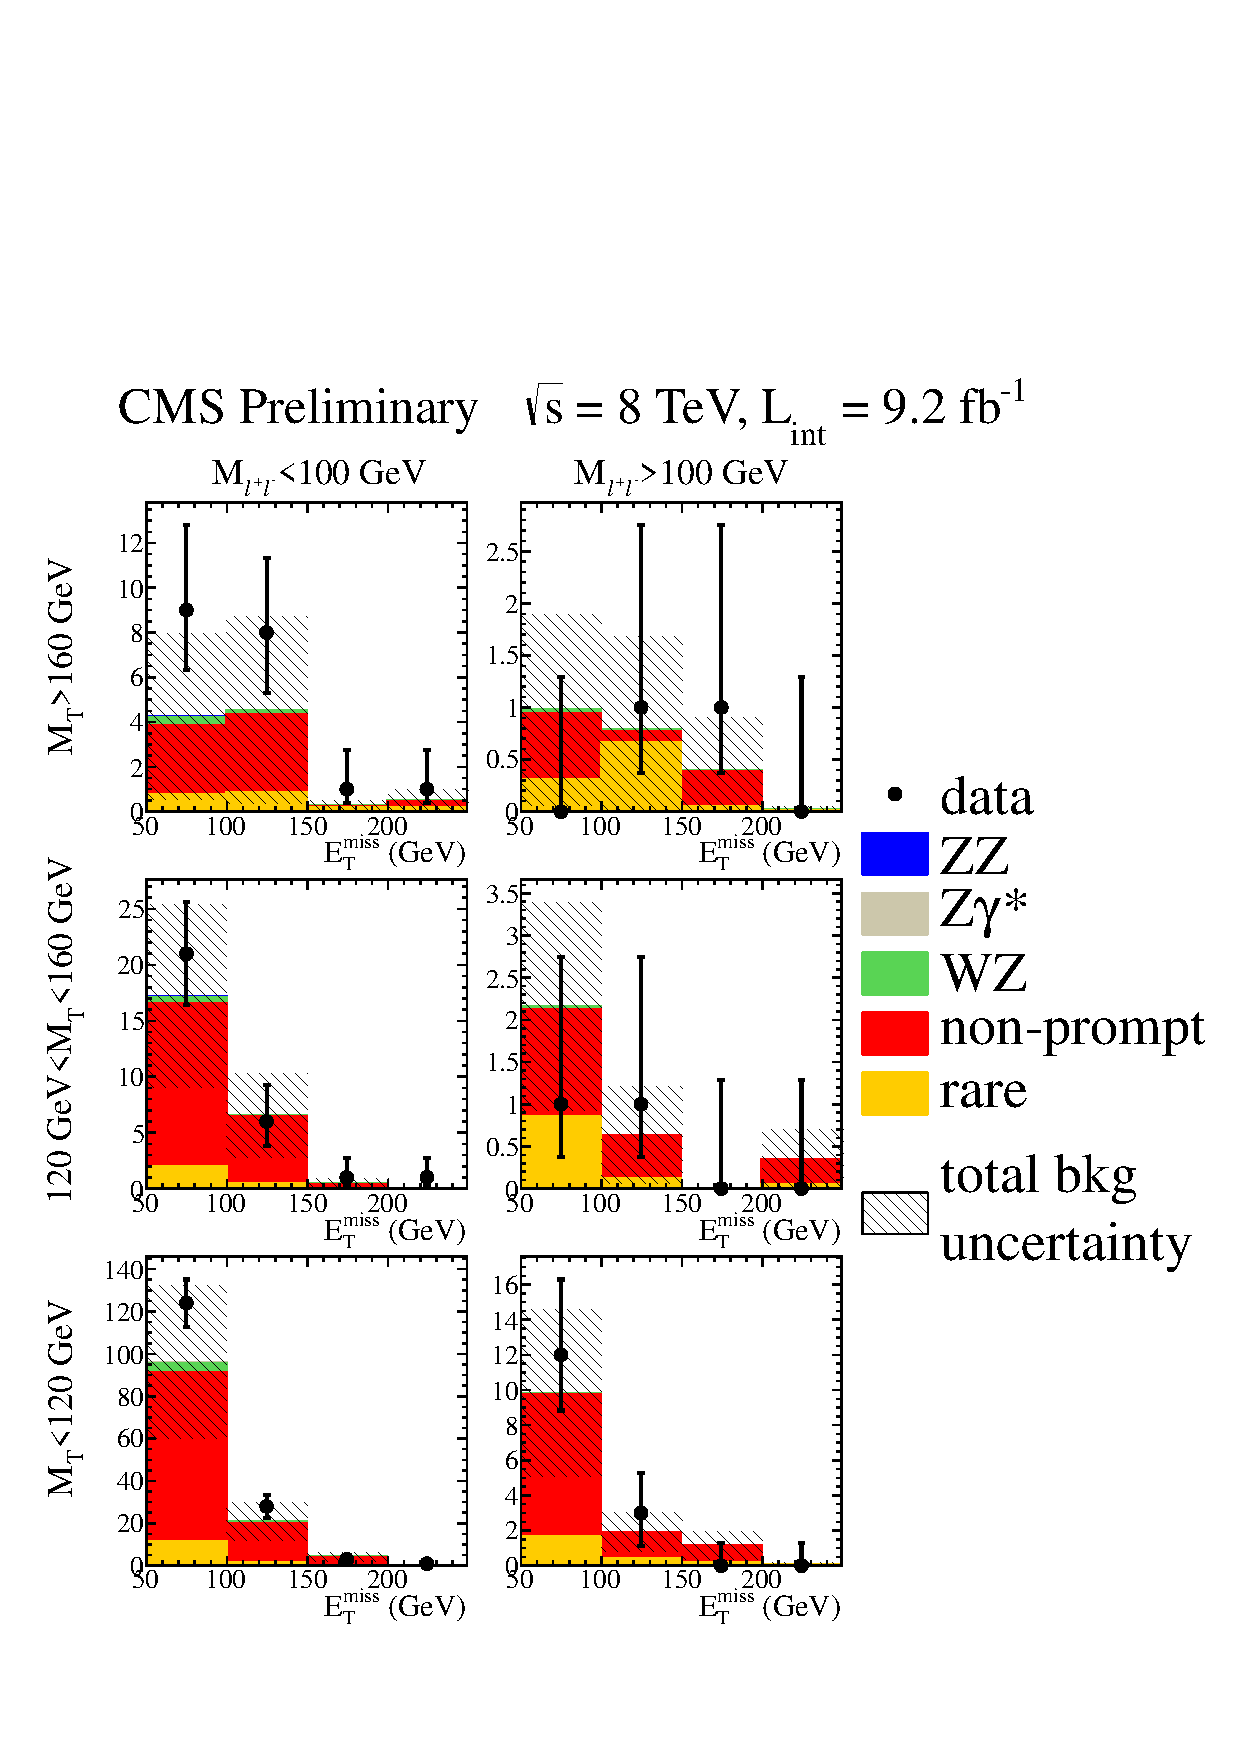
\includegraphics[width=1.0\textwidth]{plots/3lfinal/ossf0tau1_C2.pdf}
\caption{Observed yields and predicted backgrounds for a tri-lepton with an opposite sign opposite flavor di-lepton 
and a hadronically decaying tau in all defined search regions.}
\label{fig:OSOFtau1}
\end{center}
\end{figure}
%==========================================================================================%==========================================================================================
\begin{figure}[htp]
\begin{center}
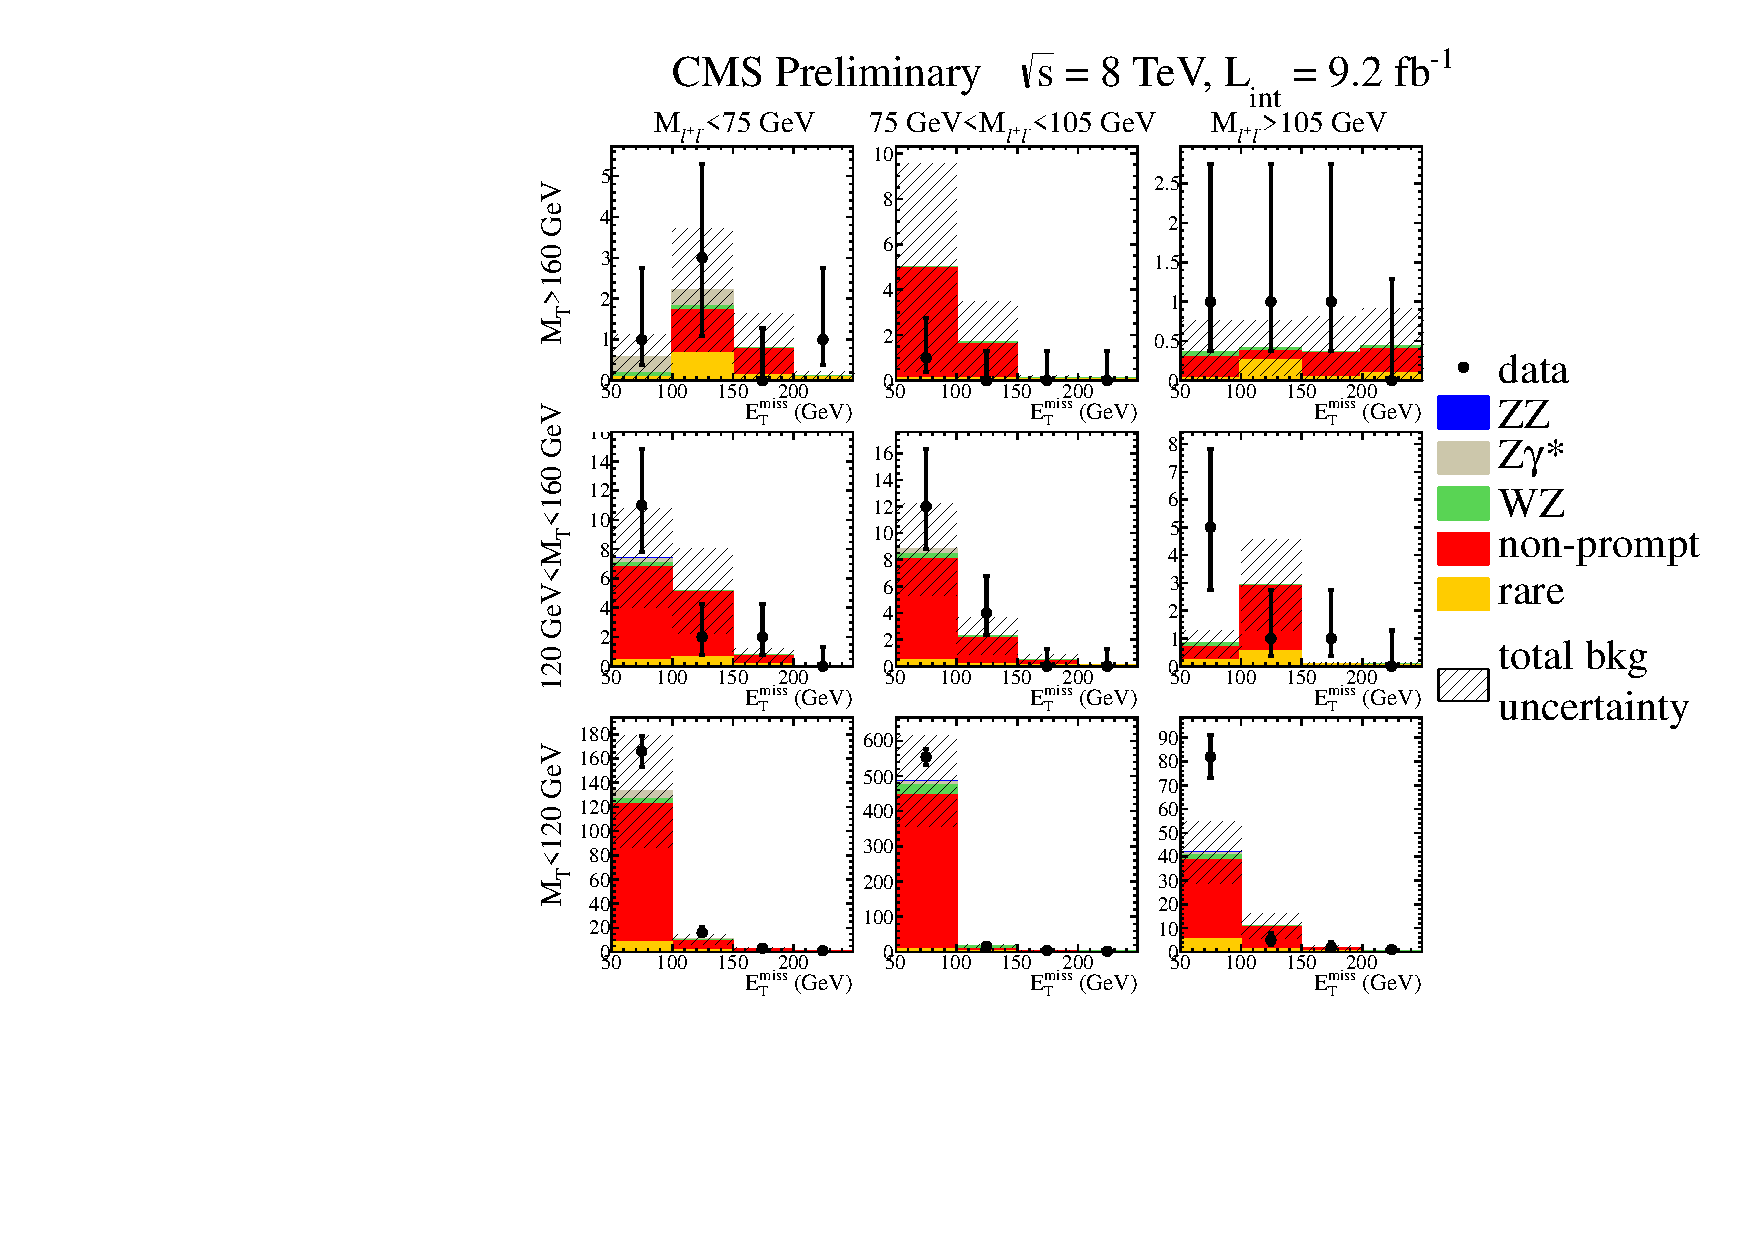
\includegraphics[width=1.0\textwidth]{plots/3lfinal/ossf1tau1.pdf}
\caption{Observed yields and predicted backgrounds for a tri-lepton with an opposite sign same flavor di-lepton 
and a hadronically decaying tau  in all defined search regions.}
\label{fig:OSSF1tau1}
\end{center}
\end{figure}
%==========================================================================================

\begin{landscape}
%==========================================================================================
%==========================================================================================
\begin{table}
%\scriptsize
\begin{center}
\caption{\label{tab:OSSF1tau0} The summary of the observed yields and predicted backgrounds for tri-lepton 
with opposite sign same flavor pair present. }
\begin{tabular}{| c | c c c c c c c | }\hline\hline
$\ETmiss$ (GeV) & WZ & Non-Prompt & Rare SM & Z$\gamma^*$ & ZZ & Total bkg & Observed\\\hline\hline
\multicolumn{8}{l}{$M_{\text{T}} > 160$ GeV, $M_{\ell\ell} < 75$ GeV}\\\hline\hline
50 -- 100&0.76$\pm$0.077&0.98$\pm$0.42&0.16$\pm$0.19&0.13$\pm$0.017&0.081$\pm$0.011&2.1$\pm$0.46&4\\
100 -- 150&0.59$\pm$0.067&0.9$\pm$0.38&0.096$\pm$0.11&0.023$\pm$0.003&0.045$\pm$0.0071&1.7$\pm$0.4&0\\
150 -- 200&0.12$\pm$0.027&0.55$\pm$0.26&0.11$\pm$0.13&0$\pm$0&0.011$\pm$0.0028&0.79$\pm$0.3&1\\
$>$ 200&0.13$\pm$0.029&0.073$\pm$0.19&0.033$\pm$0.038&0$\pm$0&0.0095$\pm$0.0025&0.25$\pm$0.2&0\\
\hline\hline
\multicolumn{8}{l}{$M_{\text{T}} > 160$ GeV, $75~\mathrm{GeV} < M_{\ell\ell} < 105~\mathrm{GeV}$}\\\hline\hline
50 -- 100&2.3$\pm$0.17&0.3$\pm$0.4&0.24$\pm$0.27&0.27$\pm$0.034&0.19$\pm$0.023&3.3$\pm$0.51&3\\
100 -- 150&1.5$\pm$0.12&0.033$\pm$0.1&0.15$\pm$0.17&0.074$\pm$0.0095&0.064$\pm$0.0094&1.8$\pm$0.23&1\\
150 -- 200&0.43$\pm$0.054&0.015$\pm$0.048&0.12$\pm$0.14&0.051$\pm$0.0065&0.015$\pm$0.0034&0.63$\pm$0.16&1\\
$>$ 200&0.19$\pm$0.035&0.27$\pm$0.14&0.11$\pm$0.12&0$\pm$0&0.007$\pm$0.0021&0.58$\pm$0.19&1\\
\hline\hline
\multicolumn{8}{l}{$M_{\text{T}} > 160$ GeV, $M_{\ell\ell} > 105$ GeV}\\\hline\hline
50 -- 100&0.46$\pm$0.058&0.11$\pm$0.02&0.5$\pm$0.66&0.13$\pm$0.016&0.025$\pm$0.0047&1.2$\pm$0.66&0\\
100 -- 150&0.19$\pm$0.034&0.16$\pm$0.31&0.49$\pm$0.61&0.21$\pm$0.026&0.011$\pm$0.0028&1.1$\pm$0.69&1\\
150 -- 200&0.083$\pm$0.022&0.033$\pm$0.068&0.14$\pm$0.17&0$\pm$0&0.0034$\pm$0.0014&0.26$\pm$0.18&0\\
$>$ 200&0.042$\pm$0.016&0$\pm$0&0.11$\pm$0.14&0.025$\pm$0.0032&0.0036$\pm$0.0015&0.18$\pm$0.14&0\\
\hline\hline
\multicolumn{8}{l}{$120~\mathrm{GeV} < M_{\text{T}} < 160~\mathrm{GeV}$, $M_{\ell\ell} < 75$ GeV}\\\hline\hline
50 -- 100&1.6$\pm$0.12&1.3$\pm$0.48&0.22$\pm$0.14&0.27$\pm$0.035&0.1$\pm$0.014&3.5$\pm$0.51&3\\
100 -- 150&0.22$\pm$0.037&0.74$\pm$0.33&0.091$\pm$0.067&0.044$\pm$0.0056&0.015$\pm$0.0033&1.1$\pm$0.34&0\\
150 -- 200&0.06$\pm$0.019&0.08$\pm$0.16&0.0046$\pm$0.0052&0$\pm$0&0.00099$\pm$0.00075&0.15$\pm$0.16&0\\
$>$ 200&0.041$\pm$0.016&0$\pm$0&0.044$\pm$0.044&0.025$\pm$0.0032&0.00078$\pm$0.00067&0.11$\pm$0.047&0\\
\hline\hline
\multicolumn{8}{l}{$120~\mathrm{GeV} < M_{\text{T}} < 160~\mathrm{GeV}$, $75~\mathrm{GeV} < M_{\ell\ell} < 105~\mathrm{GeV}$}\\\hline\hline
50 -- 100&8.7$\pm$0.48&0.61$\pm$0.27&0.25$\pm$0.15&0.16$\pm$0.021&0.4$\pm$0.048&10$\pm$0.58&11\\
100 -- 150&1.2$\pm$0.11&0.02$\pm$0.14&0.17$\pm$0.11&0$\pm$0&0.032$\pm$0.0056&1.5$\pm$0.21&0\\
150 -- 200&0.16$\pm$0.031&0.17$\pm$0.41&0.071$\pm$0.054&0$\pm$0&0.0036$\pm$0.0015&0.4$\pm$0.42&1\\
$>$ 200&0.13$\pm$0.028&0.029$\pm$0.092&0.014$\pm$0.014&0$\pm$0&0.0014$\pm$0.00089&0.17$\pm$0.097&1\\
\hline\hline
\end{tabular}
\end{center}
\end{table}
%==========================================================================================
%==========================================================================================
\begin{table*}
%\footnotesize
\begin{center}
%\caption{Continuation}
\begin{tabular}{| c | c c c c c c c | }\hline\hline
$\ETmiss$ (GeV) & WZ & Non-Prompt & Rare SM & Z$\gamma^*$ & ZZ & Total bkg & Observed\\\hline\hline
\multicolumn{8}{l}{$120~\mathrm{GeV} < M_{\text{T}} < 160~\mathrm{GeV}$, $M_{\ell\ell} > 105$ GeV}\\\hline\hline
50 -- 100&0.57$\pm$0.065&0.28$\pm$0.16&0.11$\pm$0.071&0.32$\pm$0.041&0.039$\pm$0.0064&1.3$\pm$0.19&0\\
100 -- 150&0.09$\pm$0.023&0.00033$\pm$0.00038&0.055$\pm$0.047&0.025$\pm$0.0032&0.0032$\pm$0.0014&0.17$\pm$0.053&2\\
150 -- 200&0.027$\pm$0.013&0.035$\pm$0.092&0.054$\pm$0.048&0$\pm$0&0$\pm$0&0.12$\pm$0.1&0\\
$>$ 200&0.0018$\pm$0.0043&0$\pm$0&0.077$\pm$0.086&0$\pm$0&0$\pm$0&0.079$\pm$0.086&0\\
\hline\hline
\multicolumn{8}{l}{$M_{\text{T}} < 120$ GeV, $M_{\ell\ell} < 75$ GeV}\\\hline\hline
50 -- 100&25$\pm$1.2&17$\pm$4.1&1.4$\pm$0.84&7.8$\pm$1&1.3$\pm$0.15&53$\pm$4.5&63\\
100 -- 150&3.1$\pm$0.2&2.9$\pm$0.95&0.42$\pm$0.24&0.035$\pm$0.0044&0.1$\pm$0.014&6.6$\pm$1&5\\
150 -- 200&0.83$\pm$0.081&0.36$\pm$0.2&0.19$\pm$0.13&0.015$\pm$0.0019&0.018$\pm$0.0038&1.4$\pm$0.25&1\\
$>$ 200&0.35$\pm$0.048&0.056$\pm$0.15&0.082$\pm$0.058&0.05$\pm$0.0063&0.0083$\pm$0.0024&0.54$\pm$0.17&1\\
\hline\hline
\multicolumn{8}{l}{$M_{\text{T}} < 120$ GeV, $75~\mathrm{GeV} < M_{\ell\ell} < 105~\mathrm{GeV}$}\\\hline\hline
50 -- 100&335$\pm$14.6&20.8$\pm$3.57&4.03$\pm$2.18&9.49$\pm$1.21&13.1$\pm$1.49&382$\pm$15.3&377\\
100 -- 150&58$\pm$2.8&2.3$\pm$0.82&1.8$\pm$1&0.071$\pm$0.009&1.6$\pm$0.19&63$\pm$3.1&61\\
150 -- 200&14$\pm$0.76&0.38$\pm$0.17&0.63$\pm$0.35&0.0024$\pm$0.00031&0.37$\pm$0.044&16$\pm$0.86&13\\
$>$ 200&8.7$\pm$0.49&0.045$\pm$0.085&0.55$\pm$0.3&0.031$\pm$0.0039&0.15$\pm$0.02&9.5$\pm$0.58&3\\
\hline\hline
\multicolumn{8}{l}{$M_{\text{T}} < 120$ GeV, $M_{\ell\ell} > 105$ GeV}\\\hline\hline
50 -- 100&12$\pm$0.62&4.8$\pm$1.4&1.2$\pm$0.7&0.67$\pm$0.086&0.6$\pm$0.07&19$\pm$1.7&22\\
100 -- 150&2.3$\pm$0.16&1$\pm$0.44&0.53$\pm$0.3&0.035$\pm$0.0045&0.091$\pm$0.012&4$\pm$0.56&6\\
150 -- 200&0.6$\pm$0.067&0.11$\pm$0.24&0.078$\pm$0.047&0.05$\pm$0.0064&0.029$\pm$0.0052&0.87$\pm$0.25&2\\
$>$ 200&0.36$\pm$0.05&0.028$\pm$0.054&0.029$\pm$0.02&0$\pm$0&0.014$\pm$0.0031&0.43$\pm$0.076&2\\
\hline\hline
\end{tabular}
\end{center}
\end{table*}
%==========================================================================================
%==========================================================================================
\begin{table}
%\scriptsize
\begin{center}
\caption{\label{tab:OSSF0tau0} The summary of the observed yields and predicted backgrounds for tri-lepton 
without opposite sign same flavor pair present. }
\begin{tabular}{| c | c c c c c c c | }\hline\hline
$\ETmiss$ (GeV) & WZ & Non-Prompt & Rare SM & Z$\gamma^*$ & ZZ & Total bkg & Observed\\\hline\hline
\multicolumn{8}{l}{$M_{\text{T}} > 160$ GeV, $M_{\ell\ell} < 100$ GeV}\\\hline\hline
50 -- 100&0.13$\pm$0.028&0.74$\pm$0.32&0.058$\pm$0.068&0.085$\pm$0.01&0.026$\pm$0.0048&1$\pm$0.33&1\\
100 -- 150&0.089$\pm$0.023&0.22$\pm$0.14&0.18$\pm$0.23&0.069$\pm$0.0085&0.028$\pm$0.0051&0.59$\pm$0.27&0\\
150 -- 200&0.038$\pm$0.015&0.066$\pm$0.17&0.022$\pm$0.026&0.026$\pm$0.0031&0.0037$\pm$0.0015&0.16$\pm$0.17&0\\
$>$ 200&0.038$\pm$0.015&0.0014$\pm$0.00081&0.039$\pm$0.047&0$\pm$0&0.0043$\pm$0.0016&0.083$\pm$0.049&0\\
\hline\hline
\multicolumn{8}{l}{$M_{\text{T}} > 160$ GeV, $M_{\ell\ell} > 100$ GeV}\\\hline\hline
50 -- 100&0.025$\pm$0.012&0.32$\pm$0.75&0.13$\pm$0.16&0.016$\pm$0.0021&0.0012$\pm$0.00083&0.49$\pm$0.76&0\\
100 -- 150&0.03$\pm$0.013&0.053$\pm$0.12&0.06$\pm$0.076&0.012$\pm$0.0016&0.0026$\pm$0.0012&0.16$\pm$0.14&0\\
150 -- 200&0.0034$\pm$0.0067&0.021$\pm$0.067&0.00061$\pm$0.00073&0$\pm$0&0.0014$\pm$0.00089&0.027$\pm$0.067&0\\
$>$ 200&0.017$\pm$0.0097&0$\pm$0&0.044$\pm$0.058&0.013$\pm$0.0016&0$\pm$0&0.073$\pm$0.059&0\\
\hline\hline
\multicolumn{8}{l}{$120~\mathrm{GeV} < M_{\text{T}} < 160~\mathrm{GeV}$, $M_{\ell\ell} < 100$ GeV}\\\hline\hline
50 -- 100&0.28$\pm$0.041&1.3$\pm$0.51&0.28$\pm$0.22&0.098$\pm$0.013&0.029$\pm$0.0053&2$\pm$0.56&1\\
100 -- 150&0.041$\pm$0.015&0.41$\pm$0.63&0.051$\pm$0.036&0.019$\pm$0.0025&0.0042$\pm$0.0016&0.52$\pm$0.63&1\\
150 -- 200&0.015$\pm$0.0093&0.015$\pm$0.047&0.047$\pm$0.046&0$\pm$0&0$\pm$0&0.077$\pm$0.066&1\\
$>$ 200&0.003$\pm$0.0039&0.003$\pm$0.0017&0.0068$\pm$0.0062&0$\pm$0&0$\pm$0&0.013$\pm$0.0075&0\\
\hline\hline
\multicolumn{8}{l}{$120~\mathrm{GeV} < M_{\text{T}} < 160~\mathrm{GeV}$, $M_{\ell\ell} > 100$ GeV}\\\hline\hline
50 -- 100&0.059$\pm$0.018&0$\pm$0&0.023$\pm$0.019&0.022$\pm$0.0029&0.00088$\pm$0.00071&0.11$\pm$0.026&1\\
100 -- 150&0.0037$\pm$0.0083&0.021$\pm$0.067&0.014$\pm$0.014&0.025$\pm$0.0032&0$\pm$0&0.064$\pm$0.069&0\\
150 -- 200&0$\pm$0&0$\pm$0&0.00021$\pm$0.00019&0$\pm$0&0$\pm$0&0.00021$\pm$0.00019&0\\
$>$ 200&0$\pm$0&0$\pm$0&0.004$\pm$0.0046&0$\pm$0&0$\pm$0&0.004$\pm$0.0046&0\\
\hline\hline
\multicolumn{8}{l}{$M_{\text{T}} < 120$ GeV, $M_{\ell\ell} < 100$ GeV}\\\hline\hline
50 -- 100&1.6$\pm$0.12&8.7$\pm$2.3&0.44$\pm$0.26&1$\pm$0.13&0.11$\pm$0.015&12$\pm$2.4&12\\
100 -- 150&0.27$\pm$0.042&1.8$\pm$0.6&0.29$\pm$0.18&0.18$\pm$0.023&0.01$\pm$0.0026&2.5$\pm$0.63&2\\
150 -- 200&0.079$\pm$0.022&1.7e-06$\pm$2e-06&0.062$\pm$0.05&0.012$\pm$0.0019&0.0023$\pm$0.0012&0.16$\pm$0.055&0\\
$>$ 200&0.031$\pm$0.013&0.058$\pm$0.17&0.13$\pm$0.14&0.016$\pm$0.002&0.00099$\pm$0.00075&0.24$\pm$0.22&0\\
\hline\hline
\multicolumn{8}{l}{$M_{\text{T}} < 120$ GeV, $M_{\ell\ell} > 100$ GeV}\\\hline\hline
50 -- 100&0.047$\pm$0.017&0.29$\pm$0.14&0.14$\pm$0.086&0.14$\pm$0.018&0.0021$\pm$0.0011&0.61$\pm$0.16&0\\
100 -- 150&0.0043$\pm$0.005&0.0092$\pm$0.0053&0.025$\pm$0.019&0.026$\pm$0.0033&0$\pm$0&0.065$\pm$0.02&0\\
150 -- 200&0$\pm$0&0.021$\pm$0.067&0.056$\pm$0.049&0.0083$\pm$0.0011&0.00011$\pm$0.00025&0.086$\pm$0.083&0\\
$>$ 200&0$\pm$0&0$\pm$0&0.00021$\pm$0.00017&0$\pm$0&0$\pm$0&0.00021$\pm$0.00017&0\\
\hline\hline
\end{tabular}
\end{center}
\end{table}
%==========================================================================================
%==========================================================================================
\begin{table}
%\footnotesize
\begin{center}
\caption{\label{tab:SStau1} The summary of the observed yields and predicted backgrounds for the channel 
with a same sign di-lepton and a hadronically decaying tau. }
\begin{tabular}{| c | c c c c c c c | }\hline\hline
$\ETmiss$ (GeV) & WZ & Non-Prompt & Rare SM & Z$\gamma^*$ & ZZ & Total bkg & Observed\\\hline\hline
50 -- 100&0.62$\pm$0.32&1$\pm$0.37&0.029$\pm$0.019&0$\pm$0&0.12$\pm$0.06&1.8$\pm$0.54&1\\
100 -- 150&0.3$\pm$0.15&0.25$\pm$0.14&0.17$\pm$0.11&0$\pm$0&0.05$\pm$0.025&0.77$\pm$0.31&0\\
150 -- 200&0.061$\pm$0.035&0.17$\pm$0.15&0.056$\pm$0.036&0$\pm$0&0.013$\pm$0.0071&0.3$\pm$0.17&0\\
$>$ 200&0.029$\pm$0.019&0.16$\pm$0.12&0.028$\pm$0.019&0$\pm$0&0.0065$\pm$0.0036&0.22$\pm$0.12&2\\
\hline\hline
\multicolumn{8}{l}{$M_{\text{T}} > 160$ GeV, $M_{\ell\ell} > 100$ GeV}\\\hline\hline
50 -- 100&0.034$\pm$0.021&0.18$\pm$0.12&0.009$\pm$0.0069&0$\pm$0&0.0021$\pm$0.0014&0.22$\pm$0.13&1\\
100 -- 150&0.025$\pm$0.017&0.17$\pm$0.15&0.0093$\pm$0.0069&0$\pm$0&0.0024$\pm$0.0015&0.21$\pm$0.15&1\\
150 -- 200&0$\pm$0&0.053$\pm$0.041&0.012$\pm$0.012&0$\pm$0&0.00048$\pm$0.00049&0.065$\pm$0.043&0\\
$>$ 200&0$\pm$0&0$\pm$0&0.011$\pm$0.0085&0$\pm$0&0.00027$\pm$0.00035&0.012$\pm$0.0086&0\\
\hline\hline
\multicolumn{8}{l}{$120~\mathrm{GeV} < M_{\text{T}} < 160~\mathrm{GeV}$, $M_{\ell\ell} < 100$ GeV}\\\hline\hline
50 -- 100&1.1$\pm$0.55&1.9$\pm$0.55&0.08$\pm$0.046&0$\pm$0&0.11$\pm$0.054&3.1$\pm$0.84&3\\
100 -- 150&0.12$\pm$0.062&0.39$\pm$0.19&0.027$\pm$0.018&0$\pm$0&0.0092$\pm$0.005&0.54$\pm$0.21&1\\
150 -- 200&0.02$\pm$0.014&0$\pm$0&0.0095$\pm$0.01&0$\pm$0&0.0015$\pm$0.0011&0.031$\pm$0.02&0\\
$>$ 200&0.0054$\pm$0.0058&0.022$\pm$0.023&0.0035$\pm$0.0034&0$\pm$0&0.00048$\pm$0.00049&0.032$\pm$0.024&0\\
\hline\hline
\multicolumn{8}{l}{$120~\mathrm{GeV} < M_{\text{T}} < 160~\mathrm{GeV}$, $M_{\ell\ell} > 100$ GeV}\\\hline\hline
50 -- 100&0.035$\pm$0.022&0$\pm$0&0.02$\pm$0.015&0$\pm$0&0.0014$\pm$0.001&0.056$\pm$0.033&0\\
100 -- 150&0.013$\pm$0.01&0$\pm$0&0.00015$\pm$0.00013&0$\pm$0&0$\pm$0&0.013$\pm$0.01&0\\
150 -- 200&0$\pm$0&0$\pm$0&0$\pm$0&0$\pm$0&0$\pm$0&0$\pm$0&0\\
$>$ 200&0.0065$\pm$0.0064&0$\pm$0&0$\pm$0&0$\pm$0&0$\pm$0&0.0065$\pm$0.0064&0\\
\hline\hline
\multicolumn{8}{l}{$M_{\text{T}} < 120$ GeV, $M_{\ell\ell} < 100$ GeV}\\\hline\hline
50 -- 100&7.1$\pm$3.5&25$\pm$4.6&0.43$\pm$0.22&0$\pm$0&0.46$\pm$0.23&33$\pm$6.1&25\\
100 -- 150&0.87$\pm$0.43&2.6$\pm$0.68&0.41$\pm$0.36&0$\pm$0&0.04$\pm$0.02&3.9$\pm$1&0\\
150 -- 200&0.4$\pm$0.2&0.39$\pm$0.19&0.032$\pm$0.021&0$\pm$0&0.0063$\pm$0.0036&0.82$\pm$0.29&0\\
$>$ 200&0.21$\pm$0.11&0.071$\pm$0.056&0.024$\pm$0.015&0$\pm$0&0.0033$\pm$0.002&0.31$\pm$0.14&0\\
\hline\hline
\multicolumn{8}{l}{$M_{\text{T}} < 120$ GeV, $M_{\ell\ell} > 100$ GeV}\\\hline\hline
50 -- 100&0.18$\pm$0.097&1.1$\pm$0.41&0.035$\pm$0.023&0$\pm$0&0.0072$\pm$0.0039&1.3$\pm$0.42&1\\
100 -- 150&0.025$\pm$0.017&0.25$\pm$0.11&0.02$\pm$0.014&0$\pm$0&0.0017$\pm$0.0012&0.29$\pm$0.11&0\\
150 -- 200&0.011$\pm$0.0091&0.022$\pm$0.023&0.0083$\pm$0.0065&0$\pm$0&0.0005$\pm$0.00051&0.042$\pm$0.027&0\\
$>$ 200&0.0047$\pm$0.0053&0.022$\pm$0.023&0.00011$\pm$0.00011&0$\pm$0&0$\pm$0&0.027$\pm$0.024&0\\
\hline\hline
\end{tabular}
\end{center}
\end{table}
%==========================================================================================
%==========================================================================================
\begin{table}
%\scriptsize
\begin{center}
\caption{\label{tab:OSOFtau1} The summary of the observed yields and predicted backgrounds for the channel 
with an opposite sign opposite flavor di-lepton and a hadronically decaying tau. }
\begin{tabular}{| c | c c c c c c  c | }\hline\hline
$\ETmiss$ (GeV) & WZ & Non-Prompt & Rare SM & Z$\gamma^*$ & ZZ & Total bkg & Observed\\\hline\hline
50 -- 100&0.41$\pm$0.053&6.3$\pm$2.1&0.78$\pm$0.89&0$\pm$0&0.043$\pm$0.0069&7.5$\pm$2.2&9\\
100 -- 150&0.21$\pm$0.036&4.4$\pm$1.8&0.85$\pm$0.97&0$\pm$0&0.026$\pm$0.0048&5.5$\pm$2.1&8\\
150 -- 200&0.061$\pm$0.019&0.054$\pm$0.062&0.17$\pm$0.21&0$\pm$0&0.0071$\pm$0.0022&0.3$\pm$0.22&1\\
$>$ 200&0.045$\pm$0.016&0.1$\pm$0.026&0.17$\pm$0.21&0$\pm$0&0.0059$\pm$0.0019&0.33$\pm$0.21&1\\
\hline\hline
\multicolumn{8}{l}{$M_{\text{T}} > 160$ GeV, $M_{\ell\ell} > 100$ GeV}\\\hline\hline
50 -- 100&0.027$\pm$0.013&1.6$\pm$0.58&0.31$\pm$0.36&0$\pm$0&0.0012$\pm$0.00082&1.9$\pm$0.68&0\\
100 -- 150&0.016$\pm$0.0095&0.27$\pm$0.15&0.66$\pm$0.87&0$\pm$0&0.00028$\pm$0.00039&0.95$\pm$0.89&1\\
150 -- 200&0.007$\pm$0.0064&0.23$\pm$0.24&0.055$\pm$0.072&0$\pm$0&0$\pm$0&0.29$\pm$0.25&1\\
$>$ 200&0.0088$\pm$0.0071&0.032$\pm$0.016&0.013$\pm$0.016&0$\pm$0&0.00079$\pm$0.00067&0.055$\pm$0.024&0\\
\hline\hline
\multicolumn{8}{l}{$120~\mathrm{GeV} < M_{\text{T}} < 160~\mathrm{GeV}$, $M_{\ell\ell} < 100$ GeV}\\\hline\hline
50 -- 100&0.71$\pm$0.073&16$\pm$4.6&2$\pm$1.3&0$\pm$0&0.06$\pm$0.0089&19$\pm$4.8&21\\
100 -- 150&0.076$\pm$0.021&6.1$\pm$2.5&0.51$\pm$0.33&0$\pm$0&0.0061$\pm$0.002&6.7$\pm$2.5&6\\
150 -- 200&0.022$\pm$0.011&0.18$\pm$0.044&0.035$\pm$0.029&0$\pm$0&0.0017$\pm$0.00098&0.24$\pm$0.054&1\\
$>$ 200&0.017$\pm$0.01&0$\pm$0&0.0072$\pm$0.0066&0$\pm$0&0.00098$\pm$0.00075&0.025$\pm$0.012&1\\
\hline\hline
\multicolumn{8}{l}{$120~\mathrm{GeV} < M_{\text{T}} < 160~\mathrm{GeV}$, $M_{\ell\ell} > 100$ GeV}\\\hline\hline
50 -- 100&0.02$\pm$0.011&2$\pm$0.92&0.85$\pm$0.61&0$\pm$0&0.00086$\pm$0.0007&2.8$\pm$1.1&1\\
100 -- 150&0$\pm$0&0.35$\pm$0.22&0.12$\pm$0.091&0$\pm$0&0$\pm$0&0.47$\pm$0.24&1\\
150 -- 200&0$\pm$0&0$\pm$0&6.6e-05$\pm$7.5e-05&0$\pm$0&0$\pm$0&6.6e-05$\pm$7.5e-05&0\\
$>$ 200&0$\pm$0&0.084$\pm$0.12&0.054$\pm$0.056&0$\pm$0&0$\pm$0&0.14$\pm$0.14&0\\
\hline\hline
\multicolumn{8}{l}{$M_{\text{T}} < 120$ GeV, $M_{\ell\ell} < 100$ GeV}\\\hline\hline
50 -- 100&4.28$\pm$0.268&97.8$\pm$25.4&11.7$\pm$6.37&0$\pm$0&0.232$\pm$0.0286&114$\pm$26.2&124\\
100 -- 150&0.65$\pm$0.07&19$\pm$6.4&1.8$\pm$1&0$\pm$0&0.026$\pm$0.0049&22$\pm$6.5&28\\
150 -- 200&0.16$\pm$0.032&3.7$\pm$1.5&0.37$\pm$0.26&0$\pm$0&0.006$\pm$0.0019&4.3$\pm$1.5&3\\
$>$ 200&0.12$\pm$0.026&0$\pm$0&0.14$\pm$0.098&0$\pm$0&0.0022$\pm$0.0011&0.25$\pm$0.1&1\\
\hline\hline
\multicolumn{8}{l}{$M_{\text{T}} < 120$ GeV, $M_{\ell\ell} > 100$ GeV}\\\hline\hline
50 -- 100&0.083$\pm$0.022&10$\pm$3.4&1.7$\pm$0.96&0$\pm$0&0.0096$\pm$0.0026&12$\pm$3.5&12\\
100 -- 150&0.028$\pm$0.013&2.1$\pm$0.63&0.43$\pm$0.26&0$\pm$0&0.00073$\pm$0.00064&2.5$\pm$0.68&3\\
150 -- 200&2.4e-05$\pm$3.4e-05&0.93$\pm$0.53&0.22$\pm$0.15&0$\pm$0&0$\pm$0&1.1$\pm$0.55&0\\
$>$ 200&0$\pm$0&0$\pm$0&0.095$\pm$0.073&0$\pm$0&0$\pm$0&0.095$\pm$0.073&0\\
\hline\hline
\end{tabular}
\end{center}
\end{table}
%==========================================================================================
\end{landscape}
%==========================================================================================
\begin{table}
\scriptsize
\begin{center}
\caption{\label{tab:OSSF1tau1} The summary of the observed yields and predicted backgrounds for the channel 
with an OSSF di-lepton and a hadronically decaying tau. }
\begin{tabular}{| c | c c c c c c c | }\hline\hline
$\ETmiss$ (GeV) & WZ & Non-Prompt & Rare SM & Z$\gamma^*$ & ZZ & Total bkg & Observed\\\hline\hline
\multicolumn{8}{l}{$M_{\text{T}} > 160$ GeV, $M_{\ell\ell} < 75$ GeV}\\\hline\hline
50 -- 100&0.13$\pm$0.028&0.85$\pm$0.42&0.081$\pm$0.1&0$\pm$0&0.0096$\pm$0.0026&1.1$\pm$0.44&1\\
100 -- 150&0.097$\pm$0.024&1.3$\pm$0.46&0.67$\pm$0.81&0$\pm$0&0.0049$\pm$0.0017&2.1$\pm$0.93&3\\
150 -- 200&0.04$\pm$0.015&1$\pm$0.57&0.13$\pm$0.16&0$\pm$0&0.0016$\pm$0.00097&1.2$\pm$0.59&0\\
$>$ 200&0.016$\pm$0.0095&0.061$\pm$0.031&0.091$\pm$0.11&0$\pm$0&0$\pm$0&0.17$\pm$0.12&1\\
\hline\hline
\multicolumn{8}{l}{$M_{\text{T}} > 160$ GeV, $75~\mathrm{GeV} < M_{\ell\ell} < 105~\mathrm{GeV}$}\\\hline\hline
50 -- 100&0.067$\pm$0.02&1.3$\pm$0.36&0.087$\pm$0.1&0$\pm$0&0.012$\pm$0.0029&1.5$\pm$0.37&1\\
100 -- 150&0.11$\pm$0.026&1.5$\pm$0.73&0.12$\pm$0.15&0$\pm$0&0.0073$\pm$0.0022&1.7$\pm$0.74&0\\
150 -- 200&0.036$\pm$0.015&0.0088$\pm$0.0044&0.078$\pm$0.094&0$\pm$0&0.0023$\pm$0.0012&0.13$\pm$0.095&0\\
$>$ 200&0.022$\pm$0.011&0.024$\pm$0.012&0.059$\pm$0.068&0$\pm$0&0$\pm$0&0.1$\pm$0.07&0\\
\hline\hline
\multicolumn{8}{l}{$M_{\text{T}} > 160$ GeV, $M_{\ell\ell} > 105$ GeV}\\\hline\hline
50 -- 100&0.079$\pm$0.022&0.83$\pm$0.25&0.029$\pm$0.043&0$\pm$0&0.0018$\pm$0.001&0.93$\pm$0.25&1\\
100 -- 150&0.039$\pm$0.015&0.23$\pm$0.14&0.25$\pm$0.3&0$\pm$0&0.0021$\pm$0.0011&0.52$\pm$0.33&1\\
150 -- 200&0.0071$\pm$0.0064&0.47$\pm$0.28&0.042$\pm$0.059&0$\pm$0&0.00058$\pm$0.00057&0.52$\pm$0.29&1\\
$>$ 200&0.017$\pm$0.01&0.34$\pm$0.29&0.087$\pm$0.11&0$\pm$0&0.0012$\pm$0.00082&0.44$\pm$0.31&0\\
\hline\hline
\multicolumn{8}{l}{$120~\mathrm{GeV} < M_{\text{T}} < 160~\mathrm{GeV}$, $M_{\ell\ell} < 75$ GeV}\\\hline\hline
50 -- 100&0.27$\pm$0.042&9$\pm$2.1&0.38$\pm$0.25&0$\pm$0&0.033$\pm$0.0057&9.7$\pm$2.1&11\\
100 -- 150&0.061$\pm$0.019&5.5$\pm$2&0.61$\pm$0.47&0$\pm$0&0.0031$\pm$0.0014&6.2$\pm$2&2\\
150 -- 200&0.036$\pm$0.014&0.73$\pm$0.42&0.13$\pm$0.1&0$\pm$0&0$\pm$0&0.89$\pm$0.43&2\\
$>$ 200&0.0099$\pm$0.0075&0.015$\pm$0.0074&0.019$\pm$0.021&0$\pm$0&0$\pm$0&0.044$\pm$0.024&0\\
\hline\hline
\multicolumn{8}{l}{$120~\mathrm{GeV} < M_{\text{T}} < 160~\mathrm{GeV}$, $75~\mathrm{GeV} < M_{\ell\ell} < 105~\mathrm{GeV}$}\\\hline\hline
50 -- 100&0.39$\pm$0.052&9.7$\pm$2.1&0.45$\pm$0.29&0$\pm$0&0.043$\pm$0.0068&11$\pm$2.1&12\\
100 -- 150&0.14$\pm$0.029&2.7$\pm$1.2&0.18$\pm$0.12&0$\pm$0&0.008$\pm$0.0023&3$\pm$1.2&4\\
150 -- 200&0.1$\pm$0.025&0.69$\pm$0.17&0.04$\pm$0.026&0$\pm$0&0.0042$\pm$0.0016&0.83$\pm$0.18&0\\
$>$ 200&0.032$\pm$0.014&0.2$\pm$0.35&0.044$\pm$0.036&0$\pm$0&0.00088$\pm$0.00071&0.28$\pm$0.35&0\\
\hline\hline
\multicolumn{8}{l}{$120~\mathrm{GeV} < M_{\text{T}} < 160~\mathrm{GeV}$, $M_{\ell\ell} > 105$ GeV}\\\hline\hline
50 -- 100&0.11$\pm$0.025&0.93$\pm$0.35&0.22$\pm$0.15&0$\pm$0&0.0053$\pm$0.0018&1.3$\pm$0.38&5\\
100 -- 150&0.062$\pm$0.019&2.5$\pm$0.95&0.54$\pm$0.35&0$\pm$0&0.0026$\pm$0.0012&3.1$\pm$1&1\\
150 -- 200&0.014$\pm$0.0089&0$\pm$0&0.073$\pm$0.061&0$\pm$0&0$\pm$0&0.087$\pm$0.062&1\\
$>$ 200&0.018$\pm$0.01&0.01$\pm$0.0051&0.052$\pm$0.06&0$\pm$0&0$\pm$0&0.08$\pm$0.061&0\\
\hline\hline
\multicolumn{8}{l}{$M_{\text{T}} < 120$ GeV, $M_{\ell\ell} < 75$ GeV}\\\hline\hline
50 -- 100&4.16$\pm$0.262&131$\pm$25.7&7.78$\pm$4.3&0$\pm$0&0.533$\pm$0.0627&143$\pm$26.1&166\\
100 -- 150&0.64$\pm$0.069&10$\pm$3.2&1.2$\pm$0.67&0$\pm$0&0.047$\pm$0.0073&12$\pm$3.3&16\\
150 -- 200&0.18$\pm$0.033&2.5$\pm$1&0.064$\pm$0.049&0$\pm$0&0.0054$\pm$0.0018&2.8$\pm$1&3\\
$>$ 200&0.11$\pm$0.026&0.47$\pm$0.3&0.028$\pm$0.024&0$\pm$0&0.0036$\pm$0.0015&0.61$\pm$0.3&1\\
\hline\hline
\multicolumn{8}{l}{$M_{\text{T}} < 120$ GeV, $75~\mathrm{GeV} < M_{\ell\ell} < 105~\mathrm{GeV}$}\\\hline\hline
50 -- 100&32.6$\pm$1.71&433$\pm$80.6&7.76$\pm$4.23&0$\pm$0&5.05$\pm$0.574&478$\pm$80.7&554\\
100 -- 150&7.6$\pm$0.44&7.7$\pm$2.1&0.85$\pm$0.48&0$\pm$0&0.62$\pm$0.072&17$\pm$2.2&16\\
150 -- 200&2.5$\pm$0.17&0.57$\pm$0.36&0.17$\pm$0.099&0$\pm$0&0.13$\pm$0.017&3.3$\pm$0.41&4\\
$>$ 200&1.4$\pm$0.11&0.083$\pm$0.042&0.092$\pm$0.054&0$\pm$0&0.056$\pm$0.0084&1.6$\pm$0.13&2\\
\hline\hline
\multicolumn{8}{l}{$M_{\text{T}} < 120$ GeV, $M_{\ell\ell} > 105$ GeV}\\\hline\hline
50 -- 100&2.2$\pm$0.16&40$\pm$9.5&5.4$\pm$3&0$\pm$0&0.36$\pm$0.043&48$\pm$10&82\\
100 -- 150&0.48$\pm$0.058&10$\pm$3.9&1.2$\pm$0.81&0$\pm$0&0.058$\pm$0.0087&12$\pm$4&5\\
150 -- 200&0.13$\pm$0.028&1.7$\pm$0.82&0.11$\pm$0.082&0$\pm$0&0.013$\pm$0.003&2$\pm$0.83&2\\
$>$ 200&0.063$\pm$0.019&0.14$\pm$0.068&0.059$\pm$0.042&0$\pm$0&0.0061$\pm$0.002&0.26$\pm$0.082&1\\
\hline\hline
\end{tabular}
\end{center}
\end{table}
%\end{tabular}
%\end{center}
%\end{table}
%%==========================================================================================
%\begin{table*}
%%\footnotesize
%\begin{center}
%\begin{tabular}{| c | c c c c c c c | }\hline\hline
%$\ETmiss$ (GeV) & WZ & Non-Prompt & Rare SM & Z$\gamma^*$ & ZZ & Total bkg & Observed\\\hline\hline
%==========================================================================================
%==========================================================================================
%\end{landscape}
\clearpage